\chapter{Synthetic Data}
\label{chap:sd}

Modern hand tracking systems typically employ machine learning, and the type of machine learning model usually used is a CNN \cite{mueller2017real, malik2018deephps, wang2018mask, wan2019dual, moon2018v2v}. Machine learning offers a way to solve a particular task without being explicitly programmed to perform that task. Instead, Machine Learning `learns' how to do this task by `training' on the data. This learned task is further tested on another dataset that the model did not train on to see how it performs. This idea of having a training dataset and a testing dataset is achieved in different ways. For example, in {\slshape k-fold cross validation}, $\frac{1}{k}$ of the dataset is used for testing and the remainder for training. The model is trained $k$ times with a different section of the dataset used for training and testing each time. This method is useful for evaluating the performance of a model. For the purposes of this dissertation, a simpler method of: splitting the dataset into one training and test dataset, so the model is only trained once with the training set before evaluating performance on the test set.

Synthetic data is any kind of data that is not obtained through direct empirical observation. In the context of hand tracking, real data is obtained by a camera, while synthetic data is obtained typically through graphics rendering. Ideally, any machine learning system will be trained with the same kind of data that it is going to be used for future inference, and so synthetic data should aim to replicate what a real-world camera might see as opposed to a perfect image. There are different ways in which training data is made, depending on what kind of pipeline is being used for hand tracking, but this dissertation will follow the patterns used by \cite{yuan2017bighand2, sun2015cascaded}. That is, the synthetic data that is generated consists of $K$ images and associated groundtruths (the annotation of the keypoints) describing the location of $N$ keypoints in 3D space for each image. Each depthmap image $\bm{Z}$ is an $n\times m$ matrix, where $\mathbb{Z}_{n,m} \in \mathbb{N}$ represents an individual pixel in the image, each pixel represents the depth to the nearest visible point, thus it is called a depthmap. A keypoint is a particular location of interest in the hand, such as a knuckle. An illustration of the keypoints used in this dissertation is shown in Figure \ref{fig:sd:hand}. The goal of a hand tracking system is to take $\bm{Z}$ as an input and predict $N$ 3D keypoints $\bm{\Phi}$, where $\bm{\Phi}=\{\bm{\Phi_1}, \bm{\Phi_2}, ..., \bm{\Phi_N}\}, \bm\Phi_{n} \in \mathbb{R}^{3}$. The groundtruth $\bm{Y}^i$, (where $\bm{Y}^i_n\in \bm{\Phi}$) represents the locations of $N$ keypoints in 3D Cartesian space for $K$ depthmap images in a dataset $\bm{\mathrm{D}}$, where $\bm{\mathrm{D}}_k\in\bm{Z}$. The hand tracking system is trained with a training dataset $\bm{\mathrm{D}}^t$, and is tested with a separate test dataset $\bm{\mathrm{D}}^v$. When testing the hand tracking model, the set of predictions $\bm{Y}^o$ (where $\bm{Y}^o_n\in \bm{\Phi}$) is compared with the groundtruth $\bm{Y}^i$. This comparison is performed using a performance metric $E$.

The goal of this dissertation is to train a hand tracking system on synthetic data such that it can accurately predict future keypoints from a real world sensor. The quality of the synthetic data is evaluated by training an existing hand tracking model V2V-Posenet\cite{moon2018v2v} and evaluating its performance with the synthetic dataset in comparison to a real dataset, the MSRA dataset\cite{sun2015cascaded}. To obtain a fair evaluation, the model is not modified. An assumption is made that the right and left hand are the same, all generation of a hand focusses on the right hand in this dissertation, and that the left hand can be obtained by flipping the image on the $y$-axis. The methods used to generate the synthetic data are described herein.

\section{Synthetic Data Generation Methods}
\label{sec:sdgm}
The spread, or domain of data, describes the nature of the data. In the context of hand data, this implies what kinds of hand articulations, hand shapes, and camera angles the data covers. Previous work has generally focussed on `frontal' views, where the camera is facing towards the person. The other main type of perspective for hands is the `egocentric' perspective, where the camera is facing away from the person towards the hand, an example of this is a head-mounted camera looking at the hands. Egocentric perspectives are typically harder for a hand tracking system to recognise because the possibility of self-occlusion is greater.

The MANO model is used as the model for generating synthetic data. In theory, it is possible to generate a comprehensive dataset covering all possible hand articulations, shapes, and camera positions. This is problematic in practice however for several reasons. Firstly, the question of what constitutes a comprehensive dataset is unknown, and given the dimensionality of the problem, the generation of an ever-increasingly comprehensive dataset becomes computationally infeasible for the hardware available in this dissertation (the generation method described in Section \ref{sec:sd:d} takes 607 milliseconds on average to generate a single image). The subsections herein describe two ways of generating synthetic hand data, and they both highlight the dimensionality issue. The first method sees all generation parameters determined at random, which gives a completely random dataset described in Section \ref{sec:rgm}. The other generation method attempts to recreate a real dataset using the groundtruth of that real dataset as a reference.

\subsection{Random Generation Method - {\slshape Random MANO Dataset}}
\label{sec:rgm}
\begin{figure}
    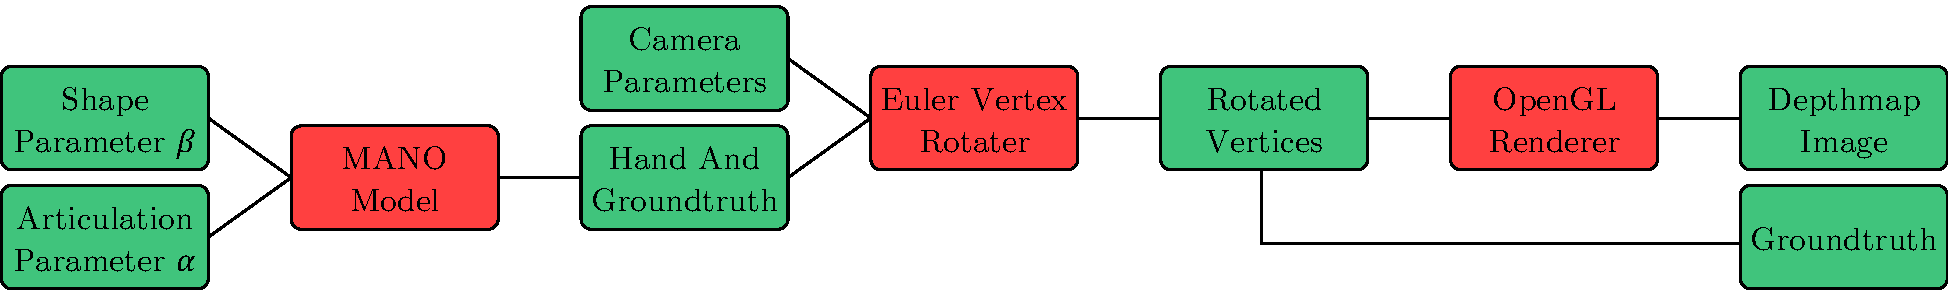
\includegraphics[width=\linewidth]{figs/general/nd_process.pdf}
    \caption{A diagram of the process for generating the Random MANO Dataset. The parameters $\alpha$, $\beta$, and camera parameters are inputs, and the depthmap image and grountruth are outputs.}
    \label{fig:ndproc}
\end{figure}
This is the first synthetic data generation strategy investigated, this dataset is called the {\slshape Random MANO Dataset}. This method involves generating an entirely random synthetic dataset, drawn from a uniform distribution, the meaning of which is described below. A diagram of this process is shown in Figure \ref{fig:ndproc}.
\subsubsection{Generating Poses and Hand Shapes}
The basic MANO model takes two parameters, $\bm{\beta} \in \mathbb{R}^{10}$ and $\bm{\theta} \in \mathbb{R}^{45}$, describing shape and articulation respectively, giving a total of 55 parameters. Following on from \cite{baek2019pushing}, The full 45-dimensional $\bm{\theta}$ parameter is used as opposed to the {\slshape principal component analysis}-based 6-dimensional subspace used in the original MANO implementation. This generates 778 vertices describing a hand based on the input parameters. The groundtruth can be obtained from an additional regressor that takes the 778 vertices as an input and outputs 16 keypoints as a grountruth. I am not aware of any a priori relationship between the input and output of this model, that is, knowing what $\bm{\beta}$ and $\bm{\theta}$ input produces a particular 778 vertex output. Given the size of the input parameters, a random number is drawn for each point $\bm{\beta}$ and $\bm{\theta}$, drawn from a uniform distribution in the range $[-2.0, 2.0]$, the range of values in-between is limited by floating point hardware alone. The underlying theory behind using this regimen is that, given a sufficient number of random draw of values for $\bm{\beta}$ and $\bm{\theta}$, they will eventually converge towards a `comprehensive' dataset insofar as the MANO model can accommodate. Giving the MANO model a zero vector for $\bm{\beta}$ and $\bm{\theta}$ returns a hand in its rest pose (the pose that the hand naturally regresses to when no muscular force is imparted on the fingers), and the greater each index in these vectors deviates from zero, the more diverse of a shape that is outputted (with fingers going in progressively more complex articulations for larger values for each index of $\bm{\beta}$ and $\bm{\theta}$). This particular range was chosen through empirical observation, a range greater than this tends to give unrealistic or impossible poses that a real hand can produce. The original MANO model keypoint regressor outputs 16 keypoints, which does not match with the 21 keypoints used with the MSRA dataset, so in this dissertation, the MANO setup for this project is taken from the code of \cite{baek2019pushing, zhang2019end}.

\subsubsection{Camera}
Before rendering the 778 vertices into a depthmap image, the camera must be set appropriately. The MANO model always generates the 778 hand vertices and 21 keypoints in the same global orientation, therefore they must be rotated afterwards to augment the dataset for different camera perspectives. The image is rendered using OpenGL, and in OpenGL, the camera is always at the zero vector $\bm{0}$ position in Cartesian space, facing in the negative $z$ direction. To manipulate the camera therefore, all of the other vertices in the scene are manipulated, and they must eventually be in the space between $[-1.0, 1.0]$ for each Cartesian axis to appear in the render\footnote{\url{https://www.khronos.org/opengl/wiki/Viewing_and_Transformations} (accessed 29th April 2020)}.

This version of the model does not include a human body, so the camera must not view the hand in any form of ego-centric perspective because the wrist is cut off from the rest of the body and a hole will be seen in the rendered hand's wrist. The groundtruth describes not only the articulation of the hand, but also the orientation and position of the hand in 3D space. To account for this, any rotation of the 778 vertices must also be performed on the 21 keypoint groundtruth. The rotations are performed using three Euler rotations in practice. Specifically, all over a uniform distribution (in radians), the $x$-axis is rotated in the range $[0, 2\pi]$ radians, the $y$-axis is rotated randomly over $[-\frac{2}{3}\pi, -\frac{1}{3}\pi]$ radians, and the $z$-axis is rotated randomly over $[\frac{2}{3}\pi, \frac{1}{3}\pi]$ radians. The 778 vertices are rendered into a depthmap $\bm{Z}$. Example images generated can be seen in Figure \ref{fig:sd:nd}.

\subsubsection{Normalisation}
\label{sec:sd:nd:norm}
The mean and variance of the rendered image need to be adjusted to match the MSRA images. The variance is scaled to the same as the average variance of the MSRA dataset, and the mean is the same as the mean value of the $z$ coordinate of each groundtruth value.

\begin{figure}
    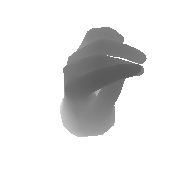
\includegraphics[width=110px]{figs/mano/0.png}
    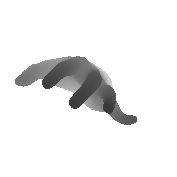
\includegraphics[width=110px]{figs/mano/1.png}
    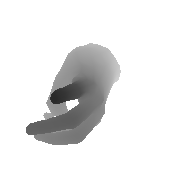
\includegraphics[width=110px]{figs/mano/2.png}
    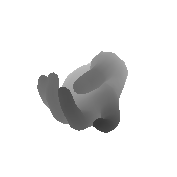
\includegraphics[width=110px]{figs/mano/3.png}
    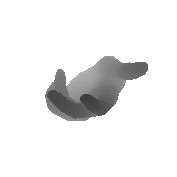
\includegraphics[width=110px]{figs/mano/4.png}
    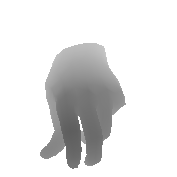
\includegraphics[width=110px]{figs/mano/5.png}
    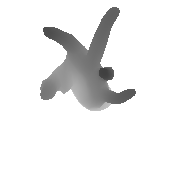
\includegraphics[width=110px]{figs/mano/6.png}
    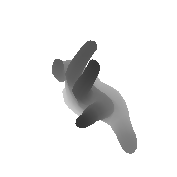
\includegraphics[width=110px]{figs/mano/7.png}
    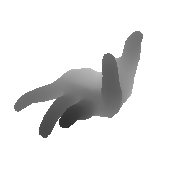
\includegraphics[width=110px]{figs/mano/8.png}
    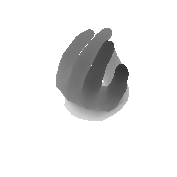
\includegraphics[width=110px]{figs/mano/9.png}
    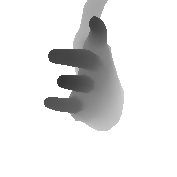
\includegraphics[width=110px]{figs/mano/10.png}
    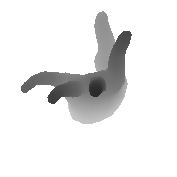
\includegraphics[width=110px]{figs/mano/11.png}
    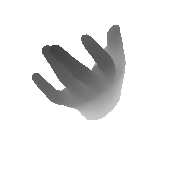
\includegraphics[width=110px]{figs/mano/12.png}
    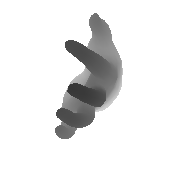
\includegraphics[width=110px]{figs/mano/13.png}
    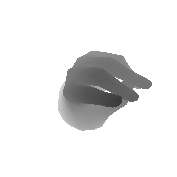
\includegraphics[width=110px]{figs/mano/14.png}
    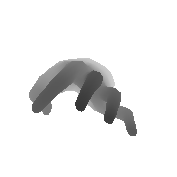
\includegraphics[width=110px]{figs/mano/15.png}
    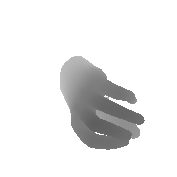
\includegraphics[width=110px]{figs/mano/16.png}
    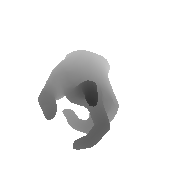
\includegraphics[width=110px]{figs/mano/17.png}
    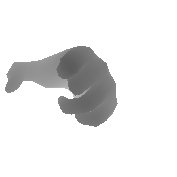
\includegraphics[width=110px]{figs/mano/18.png}
    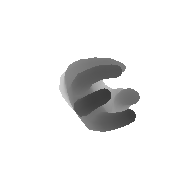
\includegraphics[width=110px]{figs/mano/19.png}
    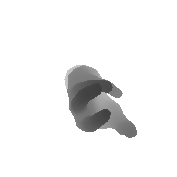
\includegraphics[width=110px]{figs/mano/20.png}
    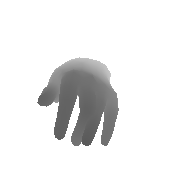
\includegraphics[width=110px]{figs/mano/21.png}
    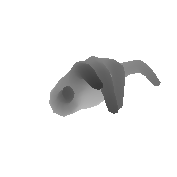
\includegraphics[width=110px]{figs/mano/22.png}
    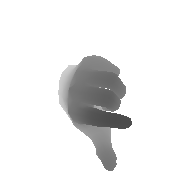
\includegraphics[width=110px]{figs/mano/23.png}
\caption{Examples of images generated using the random generation method.}
\label{fig:sd:nd}
\end{figure}

\subsection{Recreating A Real Dataset - {\slshape IK MANO Dataset}}
\begin{figure}
    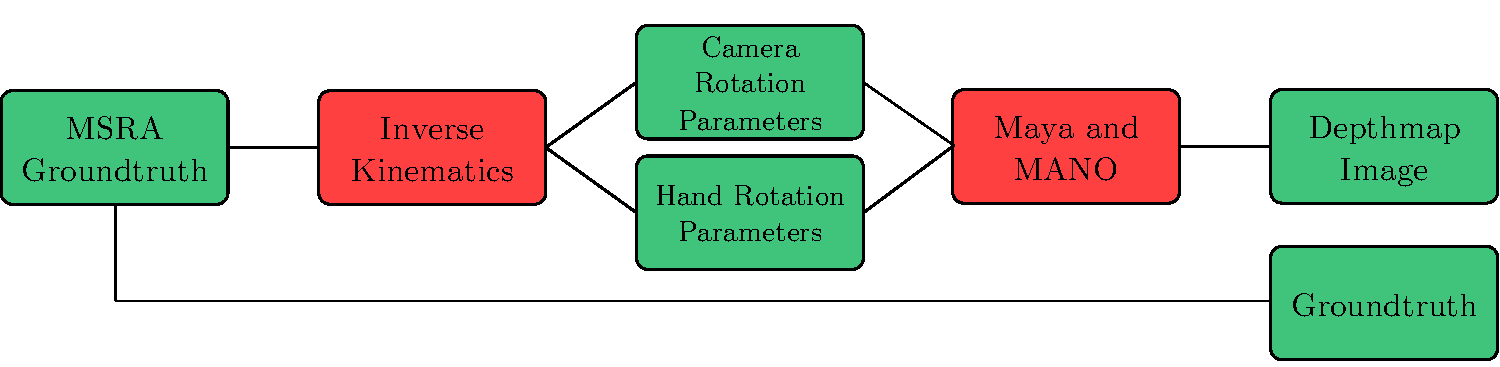
\includegraphics[width=\linewidth]{figs/general/d_process.pdf}
    \caption{A diagram of the process for producing the IK MANO Dataset. Since the recreated depth image should have the same groundtruth as the equivalent MSRA, no processing is performed on it.}
    \label{fig:dproc}
\end{figure}
\label{sec:rard}
\label{sec:sd:d}
\begin{figure}
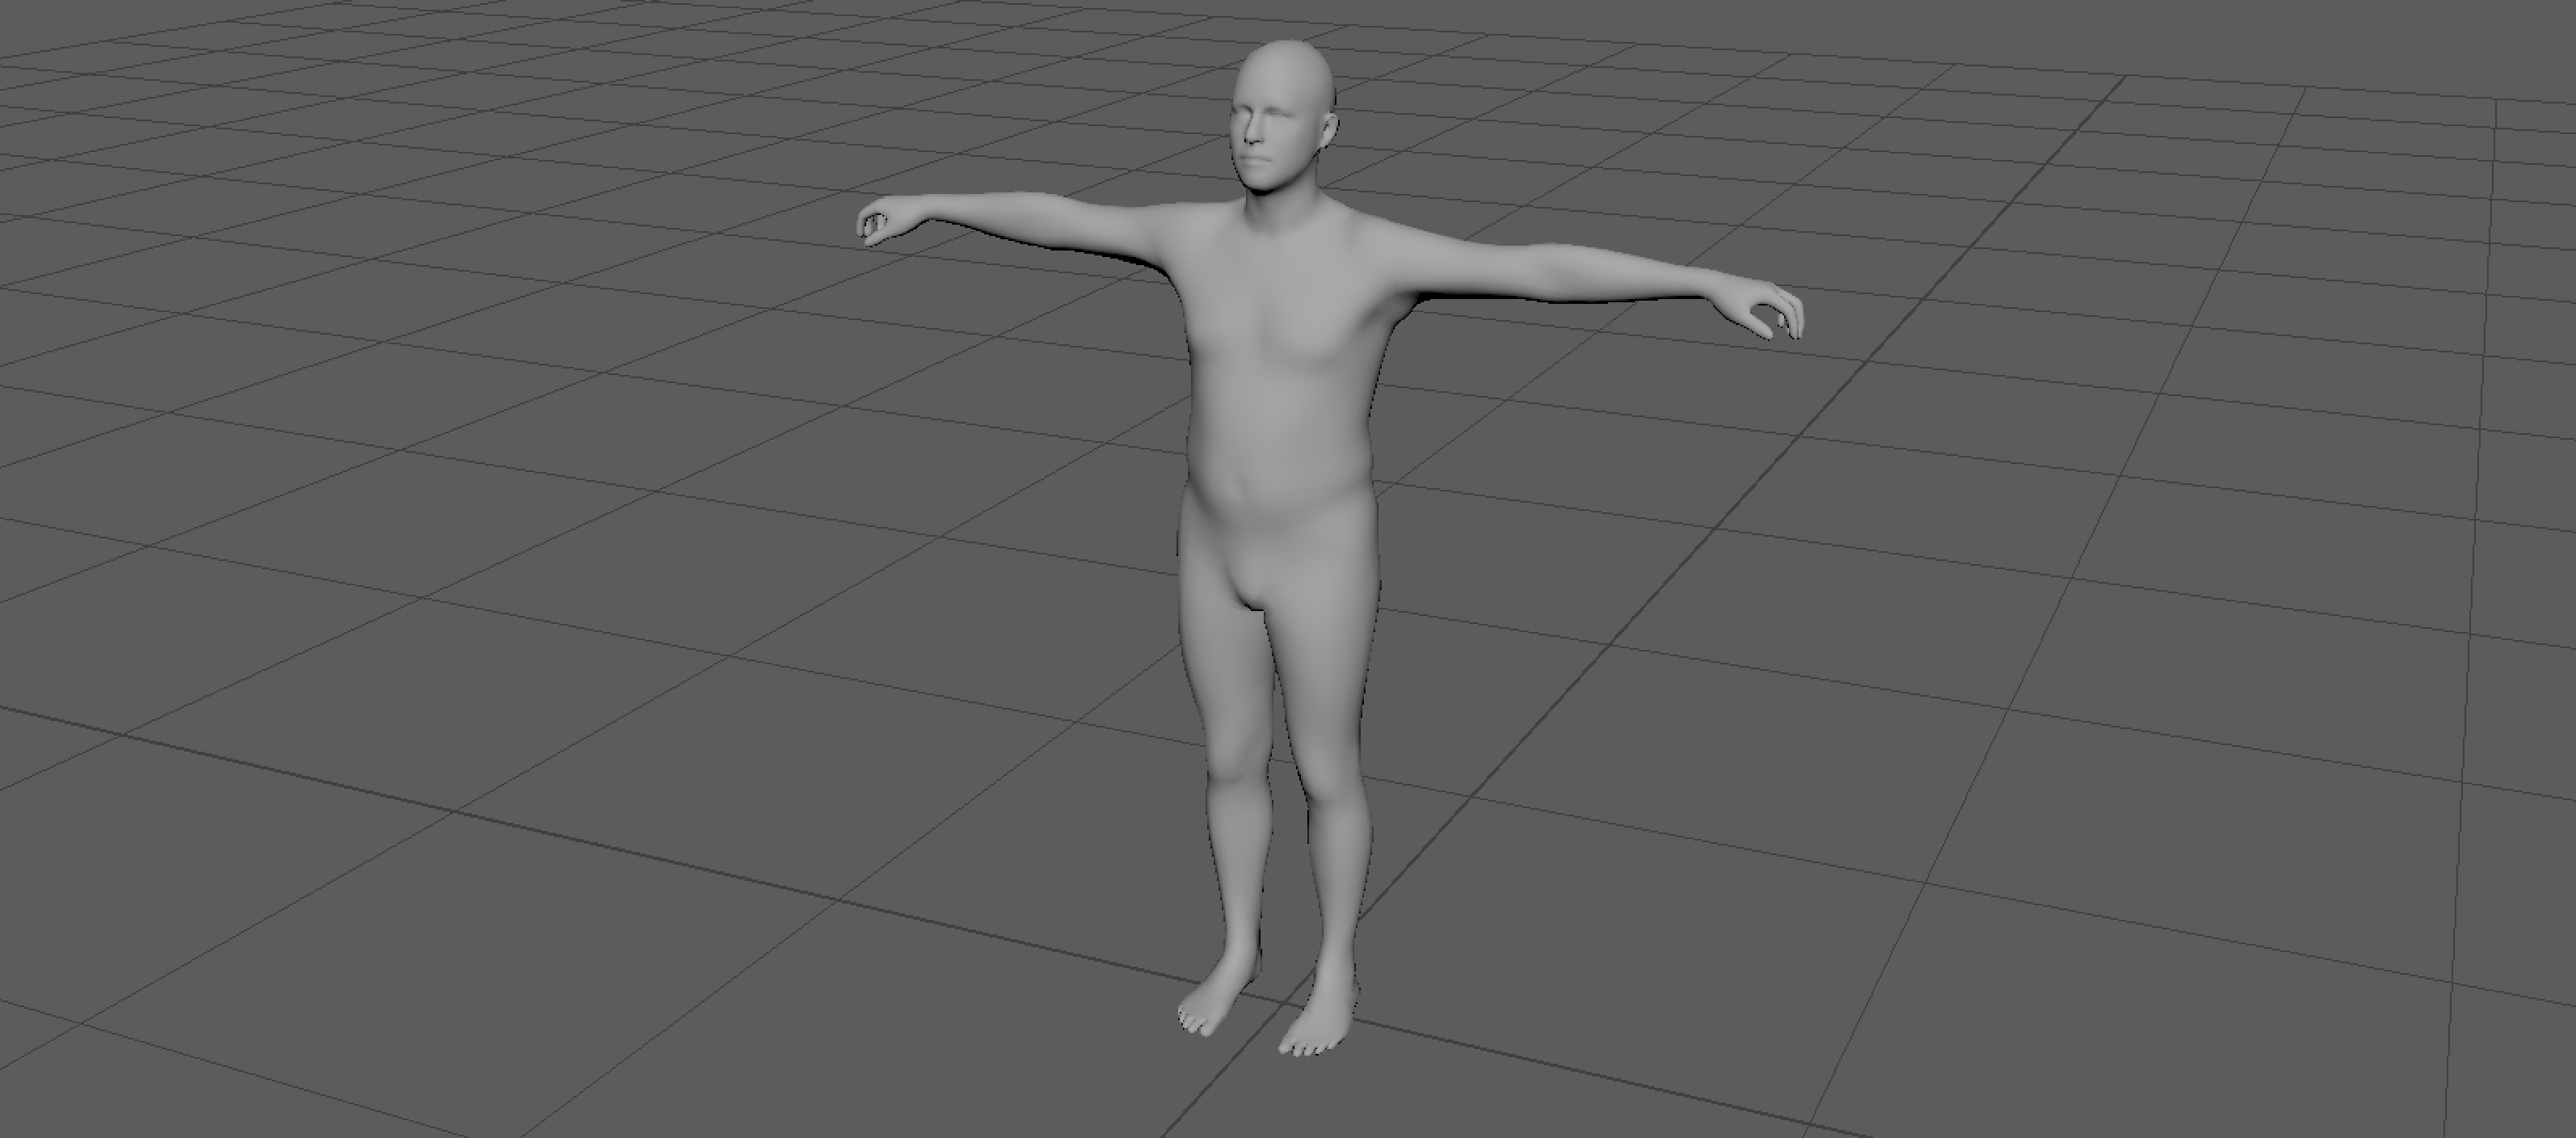
\includegraphics[width=\linewidth]{figs/general/maya.png}
\caption{Screenshot of Maya with the full body MANO model, also called SMPLH.}
\label{fig:smplh_maya}
\end{figure}

This is the second synthetic data generation strategy investigated, this dataset is called the {\slshape IK MANO Dataset}. The random data generation method described in Section \ref{sec:rgm} produces a good dataset in terms of image realism and groundtruth reliability, but it is difficult to compare with the MSRA dataset. As a reminder, the MSRA dataset \cite{sun2015cascaded} is based on certain poses within American Sign Language, and the distribution of poses likely does not match the distribution of data from the random data generation method. To address this concern, this section describes an alternative method of generating synthetic data. The goal of this method is to replicate the MSRA dataset image for image, which offers a direct way of comparing the datasets. This is a similar strategy to \cite{mueller2017real}, where they generated their synthetic data based on the hand pose estimated from a hand captured with a real sensor. To achieve this, the MANO model can be loaded into Maya (as an FBX\footnote{\url{https://www.autodesk.com/products/fbx/overview} (accessed 29th April 2020)} file) as the full human body version (specifically the male version), see Figure \ref{fig:smplh_maya}. In this setup, the hand has 16 keypoints, one for the wrist, and an MCP, PIP, and DIP joint (see Figure \ref{fig:sd:hand}), and each of these joints have three Euler rotation parameters. As well as this, each of these joints have translation parameters which can be used to change the shape of the hand, however this aspect is outside the scope of this dissertation. For hand articulation alone, this gives 45 rotation parameters, which is grossly overconstrained, since it allows us to deform the hand in ways that are not possible for a human. As mentioned in \cite{malik2018deephps}, having implausible hand images might not necessarily be detrimental towards a hand tracking system, however since the purpose of this is to recreate a dataset, this is not be a problem regardless. The following paragraphcs describes the process for reverse engineering the MSRA groundtruth for the purposes of deforming the hand articulation, and how the camera is adjusted to recreate the same camera perspective as the MSRA dataset.

\subsubsection{Extracting hand articulation information from MSRA groundtruth}
\label{sec:sd:d:ex}
There is not a simple mapping from 21 keypoints to 15 finger joint rotations, therefore a mapping needs to be determined to find rotations of the finger to manipulate the MANO model in Maya. Formally, this process is Inverse Kinematics, a subset of Robotics. Human hands though are different to robots since the bone lengths of the MANO model and annotations are different. Taking advantage of the fact that the MSRA dataset includes an annotation for the tip of the finger, the property of the dot product ($\bm{a}\cdot\bm{b}=||\bm{a}||\,||\bm{b}||\cos{\alpha}$) is used to convert the 21 MSRA joint annotation to 15 finger rotations, in a similar way to how rotations are calculated in the {\slshape Cyclic Coordinate Descent Method}\cite{fedor2003application}. These rotations are then used to deform the hand model within Maya. Two joint vectors are subtracted from each other to produce a `phalanx vector' describing the vector orientation between the two joints in consideration, this is described in Equation \ref{eq:dotproduct}. To assist in mapping equation \ref{eq:dotproduct} to the finger rotations in Maya, it is used under the following assumption:

\begin{enumerate}
    \item The palm of the hand (the region between the MCP joints and the wrist) is a rigid body.
    \item All MCP joints have two degrees of freedom - $x$-axis and $y$-axis.
    \item All PIP and DIP joints have one degree of freedom - $x$-axis only.
    \item The four finger MCP joints form a perfectly straight line in 3D space
\end{enumerate}

For simplicity, the wrist is also considered to be a joint. Figure \ref{fig:sd:ikvis} provides an illustration of this process, for example, the vectors $\bm{\Phi}_a$, $\bm{\Phi}_b$, and $\bm{\Phi}_c$ could represent the 3D locations of the MCP, PIP, and DIP respectively for the index finger, and the angle formed by Equation \ref{eq:dotproduct} is the angle that the index finger is deformed at the index PIP joint in the $x$-axis. An enumerated list of rotations performed in the $x$-axis can be found in Table \ref{tb:xrots}.

As stated above, the MCP joint is also assumed to rotate in the $y$-axis, those rotations are calculated as follows. For the pinky finger, index finger, and thumb, their respective PIP and MCP joints are used in conjunction with the next MCP joint. For the middle and ring fingers, this is used for MCP joints on either side, and whichever adjoining combination produces a larger angle in absolute terms is used. See Table \ref{tb:yrots} for a fuller explanation.

\begin{figure}
    \centering
    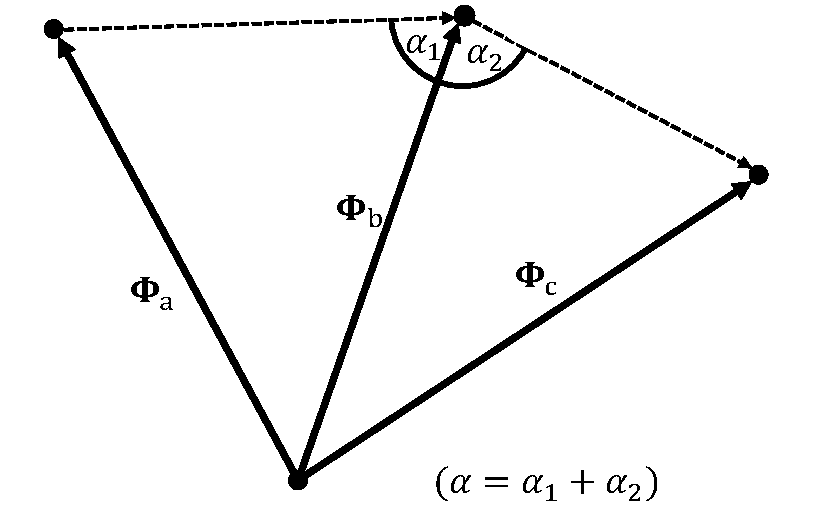
\includegraphics[width=8cm]{figs/general/ik.pdf}
    \caption{A visualisation of how the rotation of a joint is found. $\bm{\Phi}_a$, $\bm{\Phi}_b$, and $\bm{\Phi}_c$ are passed to Equation \ref{eq:dotproduct} to find the angle $\alpha$.}
    \label{fig:sd:ikvis}
\end{figure}

\begin{equation}
    \alpha = \arccos\Bigg({\frac{(\bm{\Phi}_c - \bm{\Phi}_b) \cdot (\bm{\Phi}_b - \bm{\Phi}_a)}{||\bm{\Phi}_c - \bm{\Phi}_b||\,\, ||\bm{\Phi}_b - \bm{\Phi}_a||}}\Bigg)
    \label{eq:dotproduct}
\end{equation}

% \chapter{Enumerated List of Rotations}

% \FloatBarrier\section{}
% \label{sec:ap:enumrotations}
\begin{table}[!ht]
    \centering
    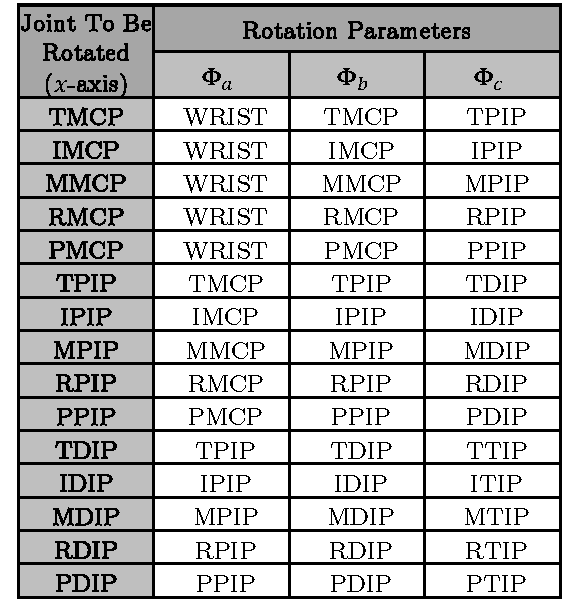
\includegraphics{figs/general/x_rots.pdf}
    \caption{Fully enumerated list of how each joint was rotated in the \underline{{\bfseries $\bm{x}$-axis}} for the inverse kinematics algorithm. See Equation \ref{eq:dotproduct} in Section \ref{sec:sd:d:ex}. See Figure \ref{fig:sd:hand} for details on the joint names.}
    \label{tb:xrots}
\end{table}

\begin{table}[]
    \centering
    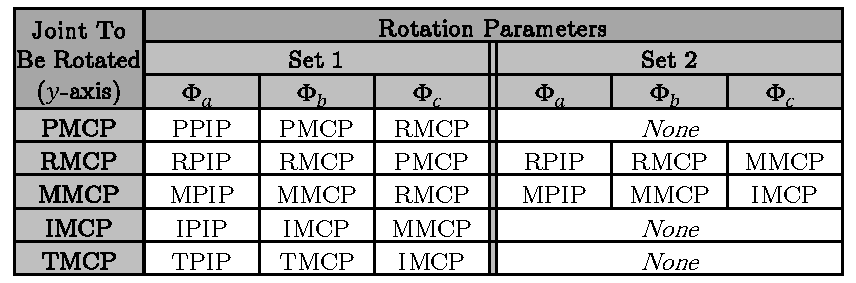
\includegraphics{figs/general/y_rots.pdf}
    \caption{Fully enumerated list of how each joint was rotated in the \underline{{\bfseries $\bm{y}$-axis}} for the inverse kinematics algorithm. See Equation \ref{eq:dotproduct} in Section \ref{sec:sd:d:ex}. Where a joint to be rotated has two sets of $\bm{\Phi}_a$, $\bm{\Phi}_b$, and $\bm{\Phi}_c$ vectors, the combination that produces the greatest magnitude of $\alpha$ in absolute terms with Equation \ref{eq:dotproduct} is chosen. See Figure \ref{fig:sd:hand} for details on the joint names.}
    \label{tb:yrots}
\end{table}

To calculate the $x$ rotations for each MANO joint, the corresponding MSRA joint, as well as the previous and next joint is used in the above formula. For example, to calculate the $x$ rotation for the PIP rotation of the ring finger, the RMCP, RPIP, and RDIP joints are inputted into Equation \ref{eq:dotproduct} letting $\bm{\Phi}_a=$RMCP, $\bm{\Phi}_b=$RPIP, and $\bm{\Phi}_c=$RDIP.

% \subsection{Hand shape}
% The shape of the hand can be changed by changing the Cartesian coordinates of each joint in the hand.

\begin{figure}
    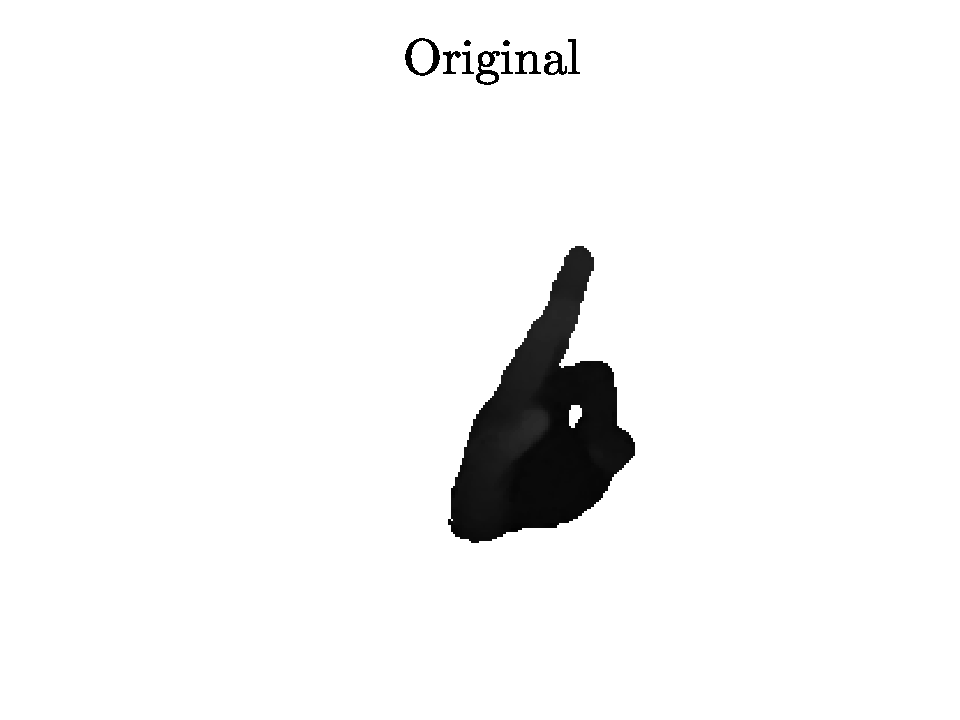
\includegraphics[width=0.48\linewidth]{figs/d_mano/original1.pdf}
    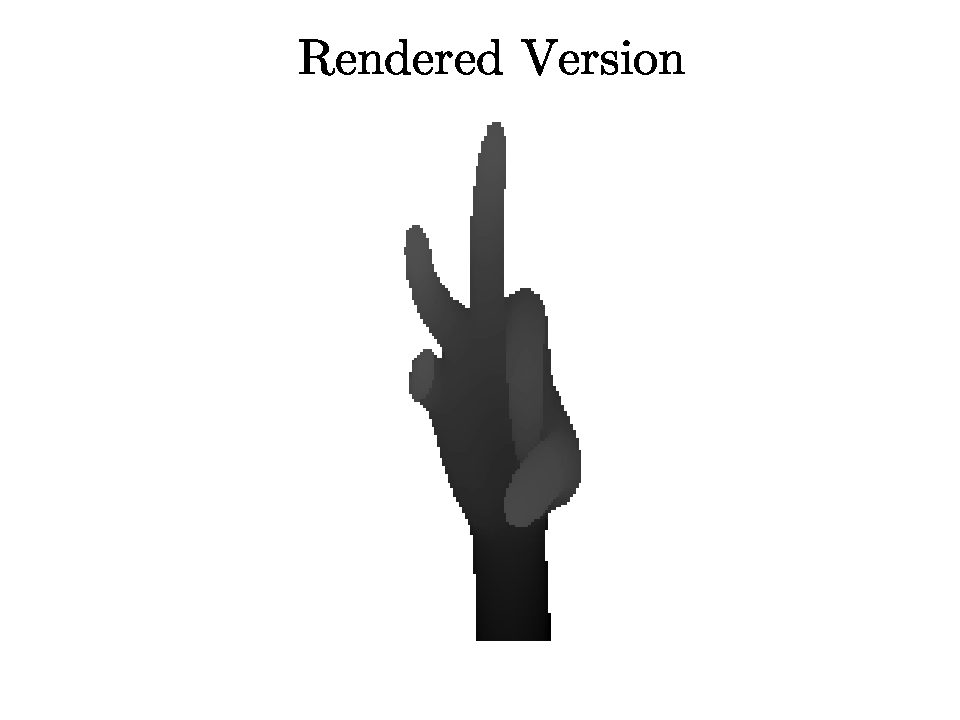
\includegraphics[width=0.48\linewidth]{figs/d_mano/rendered1.pdf}
    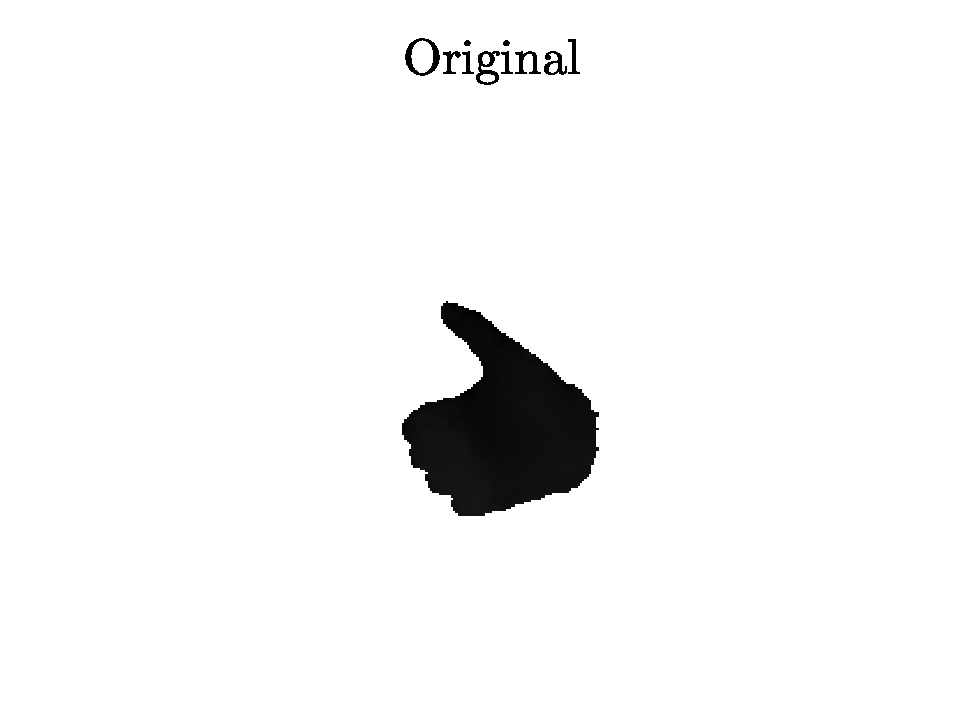
\includegraphics[width=0.48\linewidth]{figs/d_mano/original2.pdf}
    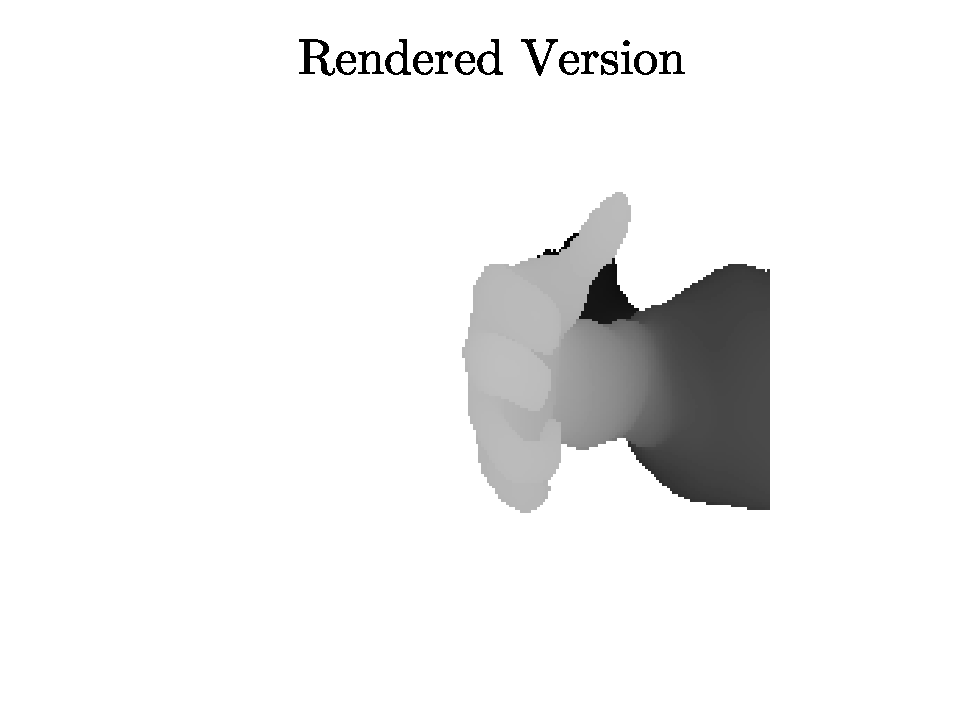
\includegraphics[width=0.48\linewidth]{figs/d_mano/rendered2.pdf}
    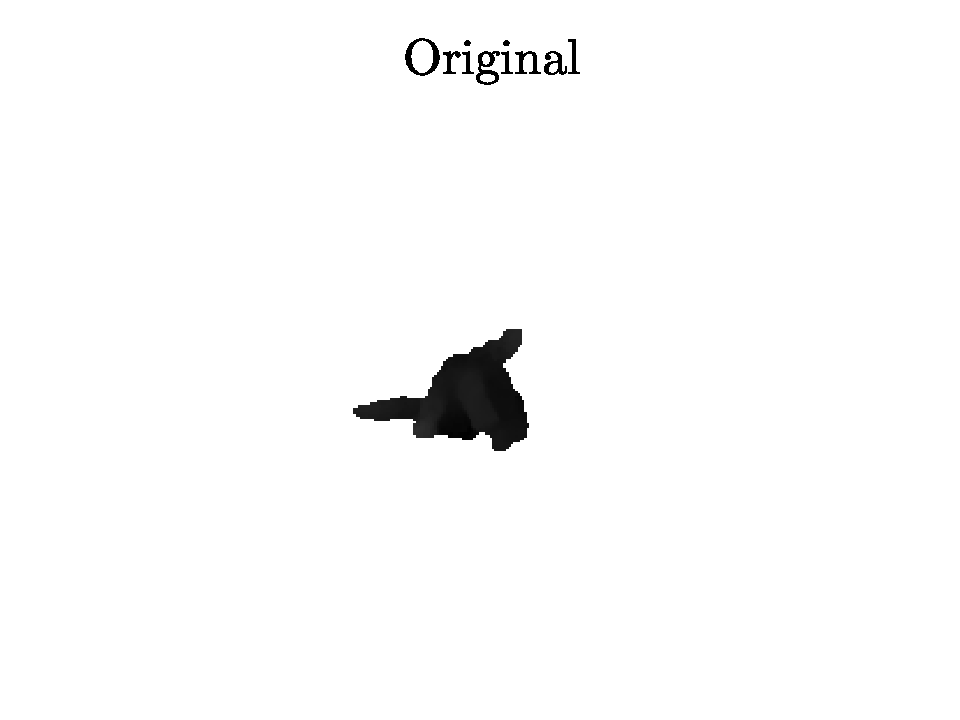
\includegraphics[width=0.48\linewidth]{figs/d_mano/original3.pdf}
    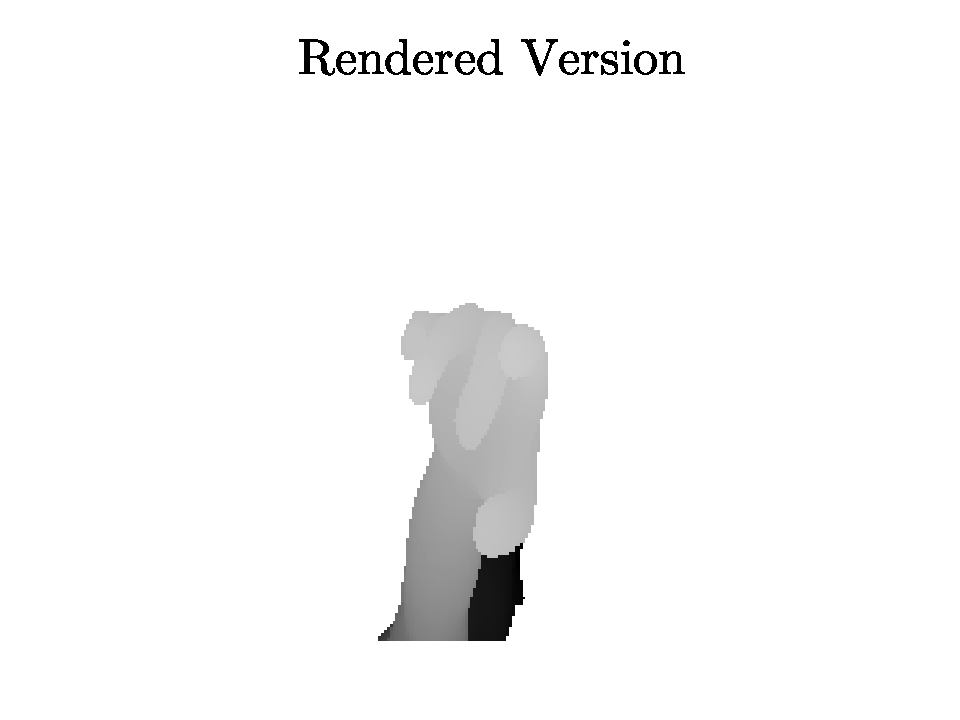
\includegraphics[width=0.48\linewidth]{figs/d_mano/rendered3.pdf}
    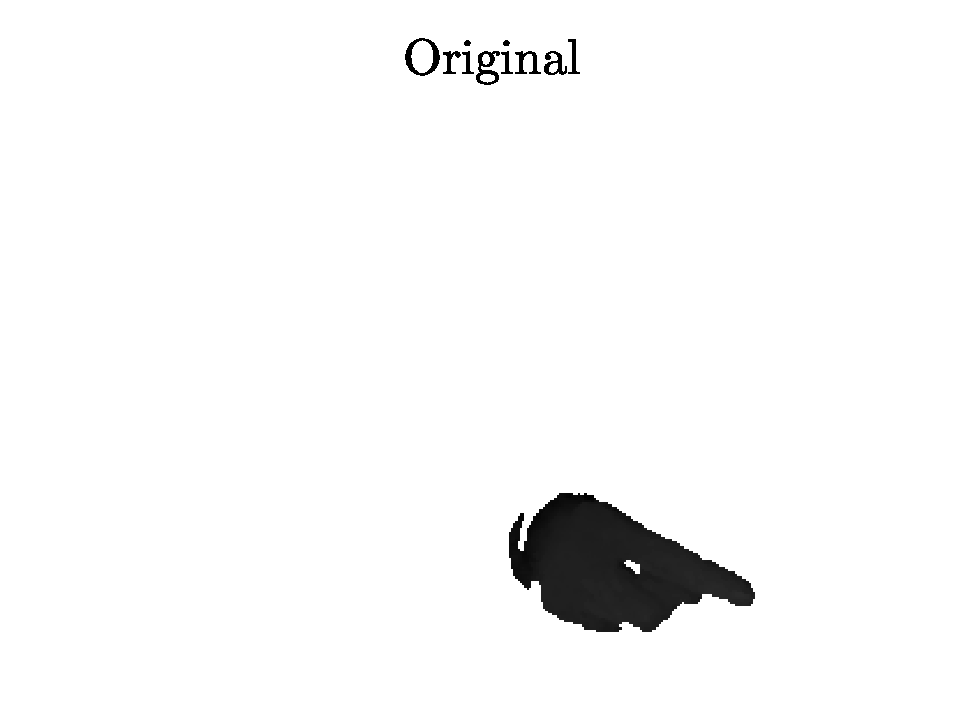
\includegraphics[width=0.48\linewidth]{figs/d_mano/original4.pdf}
    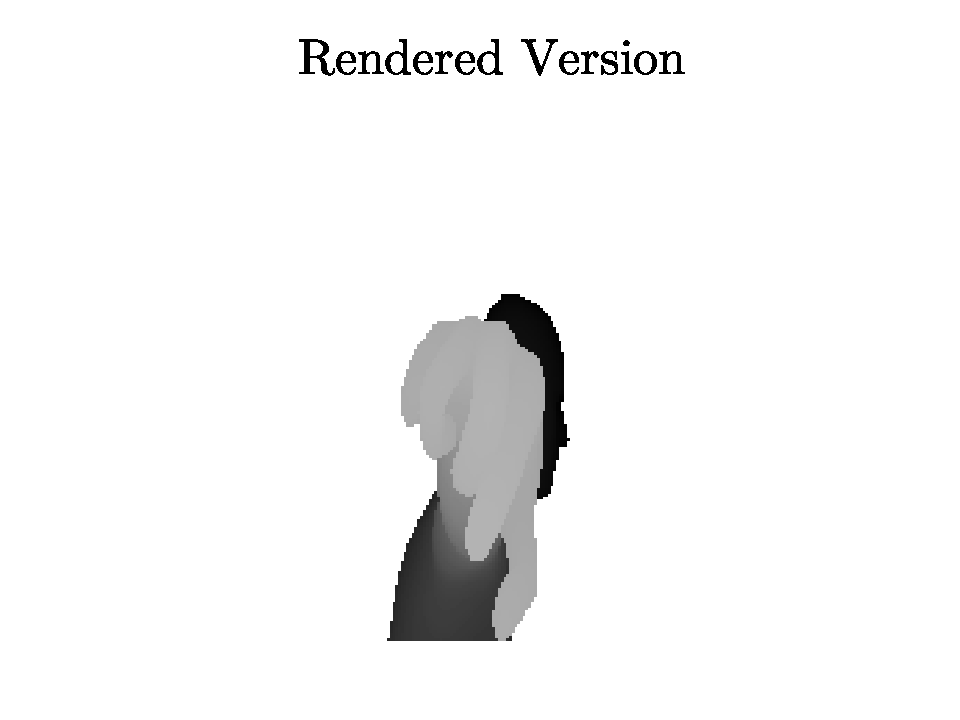
\includegraphics[width=0.48\linewidth]{figs/d_mano/rendered4.pdf}
    % 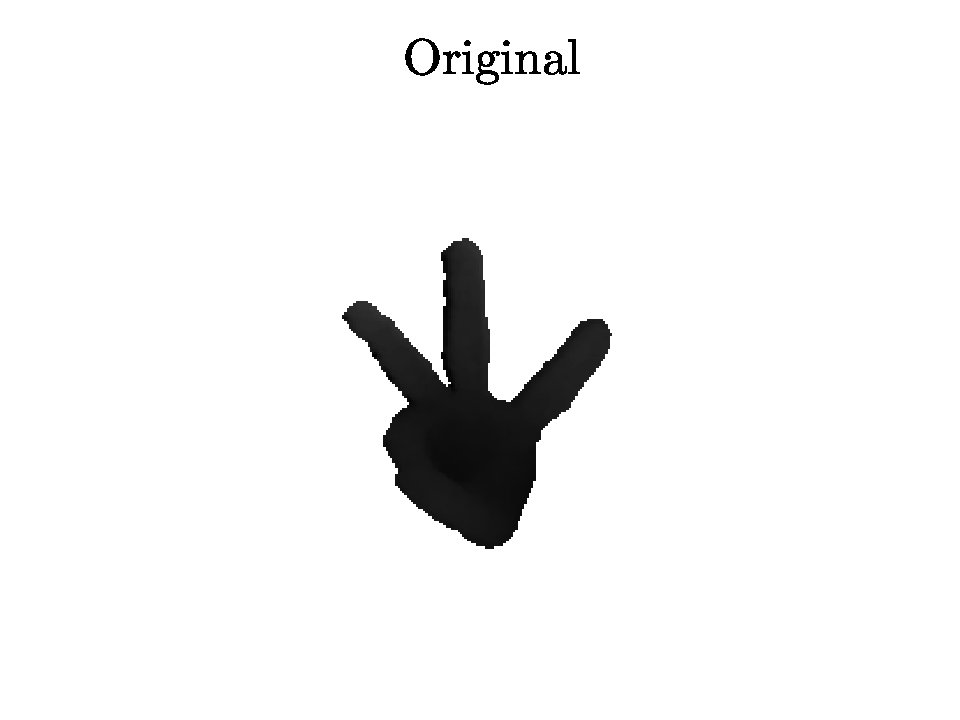
\includegraphics[width=220px]{figs/d_mano/original5.png}
    % 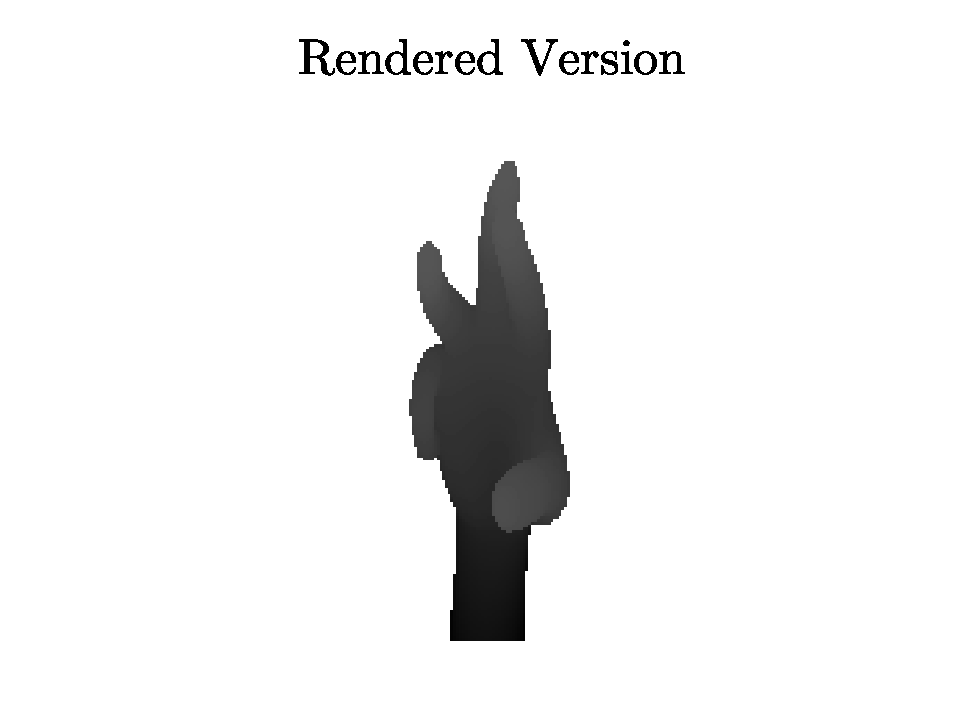
\includegraphics[width=220px]{figs/d_mano/rendered5.png}
\caption{Examples of images generated by trying to recreate the MSRA dataset. Note that the difference in colour is not significant and is dependent on the visualisation method only. The visible body is also segmented in training.}
\label{fig:sd:d}
\end{figure}

\subsubsection{Camera}
\label{sec:sd:d:cam}
The camera in Maya is the point in the scene where the renderer views from. It takes six parameters, three for Cartesian coordinates, and three for rotation: roll, pitch, and yaw ($\bm{R}_x$, $\bm{R}_y$, and $\bm{R}_z$). The camera for generating synthetic data is focused on the palm of the hand. The radius is set to a constant value, and the camera is always pointing towards a fixed point in the palm of the hand $P$, and it is moved by giving it the pitch, roll, and yaw parameters.

To achieve this, the camera is initially placed at point $[0, 0, r]$, where $r$ is the distance to the palm of the hand. Using the three rotation parameters, this point is rotated on the $x$, $y$, and $z$ axes by $\bm{R}_x$, $\bm{R}_y$, and $\bm{R}_z$ respectively. That rotated point is then translated to look at the hand by summing it by $P$, the resultant value is the new position in 3D space for the camera. The camera is then rotated by the same parameters $\bm{R}_x$, $\bm{R}_y$, and $\bm{R}_z$. This means that the camera will always be focused on the hand regardless of the input parameters $\bm{R}_x$, $\bm{R}_y$, and $\bm{R}_z$. The values of $\bm{R}_x$, $\bm{R}_y$, and $\bm{R}_z$ are obtained thus. The wrist and Index MCP coordinates are subtracted from each other to get a 3D vector describing the global rotation of the hand. The $x$, $y$, and $z$ rotations are then found using the right-angled triangle definition $\alpha=\arctan{\frac{a}{b}}$. The hyperparameters for this method were optimised by iterating over different values. This iterative method works by generating a small dataset (e.g. 1000 images), and testing the performance on the V2V-Posenet model that has been trained on the MSRA dataset.

This method does not robustly recreate the camera perspective found in the MSRA dataset, and unfortunately, the original MSRA dataset does not contain camera data.

\subsubsection{Normalising rendered image}
The process is the same as is described in Section \ref{sec:sd:nd:norm}.

\section{Transfer Learning}
% TODO: Correct MSRA count
\begin{figure}
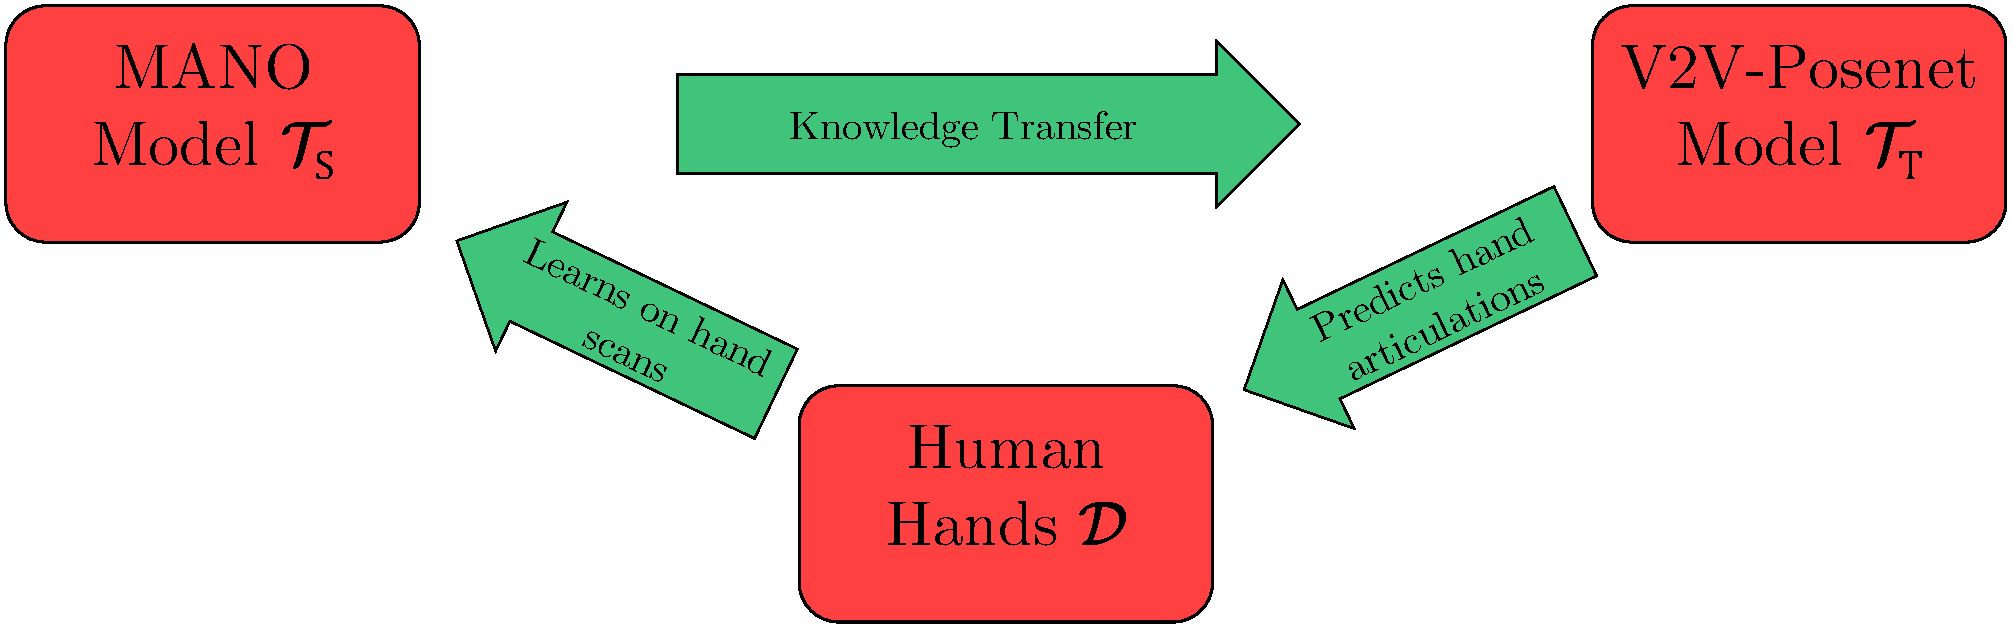
\includegraphics[width=\linewidth]{figs/general/knowledge_transfer.pdf}
\caption{High level overview of knowledge transfer in terms of training a hand tracking model using a synthetic hand generator. A task is denoted by $\mathcal{T}$, and a domain of data is denoted by $\mathcal{D}$.}
\label{fig:ktex}
\end{figure}
Formally, training a hand tracking system on synthetic data is a form of Transfer Learning, or knowledge transfer. Transfer learning is the idea of transferring the knowledge gained from training one model to another model \cite{pan2009survey}. The theory is that although the two tasks may be different, there may be some aspects of that knowledge that can be transferred, which reduces the need for new expensive labelled data. For example, if a CNN model has been trained to find if there are cars in an image, when training a CNN system to find if there are lorries in the image, there might be aspects of the knowledge in the car classification model that can be transferred to the lorry classification model. In practice, an example of how that can be achieved is by reusing the weights of some of the layers in the car CNN for the truck CNN and training only the end layers of that truck CNN. The key questions for Transfer Learning are: when should this approach be used, what knowledge should be transferred, and how should this be done in practice.

% Potentially bullshitting here
% The concept of what knowledge is is a notoriously vague topic, and this dissertation is not about Epistemology. However the topic is slightly easier to grasp when referring to data. Data and knowledge are different, and it is arguable that one of the main purposes of a computer is to gain knowledge from data. That is why certain computing tasks such as hand tracking are difficult. We as humans can observe an image of a hand and instantly know what the hand is doing, this knowledge is stored as data in the form of an image, but for a computer to extract this same knowledge is not so easy. The previous section has discussed many of the advances made in hand tracking, but they all using some form of CNN, and for the most part, we do not know how they work, because we don't know how the knowledge of a hand is encoded in the data of an image.

It is important to distinguish transfer learning from machine learning. In machine learning, a task is learned {\slshape from scratch} with training data. A successful machine learning task will train a model entirely on a dataset that is within the domain of the future examples that it is trying to predict. Using the example in Figure \ref{fig:mlex}, this model has learned to classify data into classes {\slshape red}, {\slshape green}, and {\slshape blue}. It learns these classifications given input data $x_1$ and $x_2$. Mathematically, this model can predict data from any domain, but it is only likely to be correct for data that it learned from. For example, the point marked with `?' lies in an ambiguous domain space, and we cannot be sure what class it belongs to. In contrast, in this dissertation the knowledge of the hand has already been learned in the MANO model, and the task is simply to transfer that knowledge to the V2V-Posenet model, the goal is to be able to train the V2V-Posenet model to learn from synthetic data without ever having to use real data.

\begin{figure}[H]
    \centering
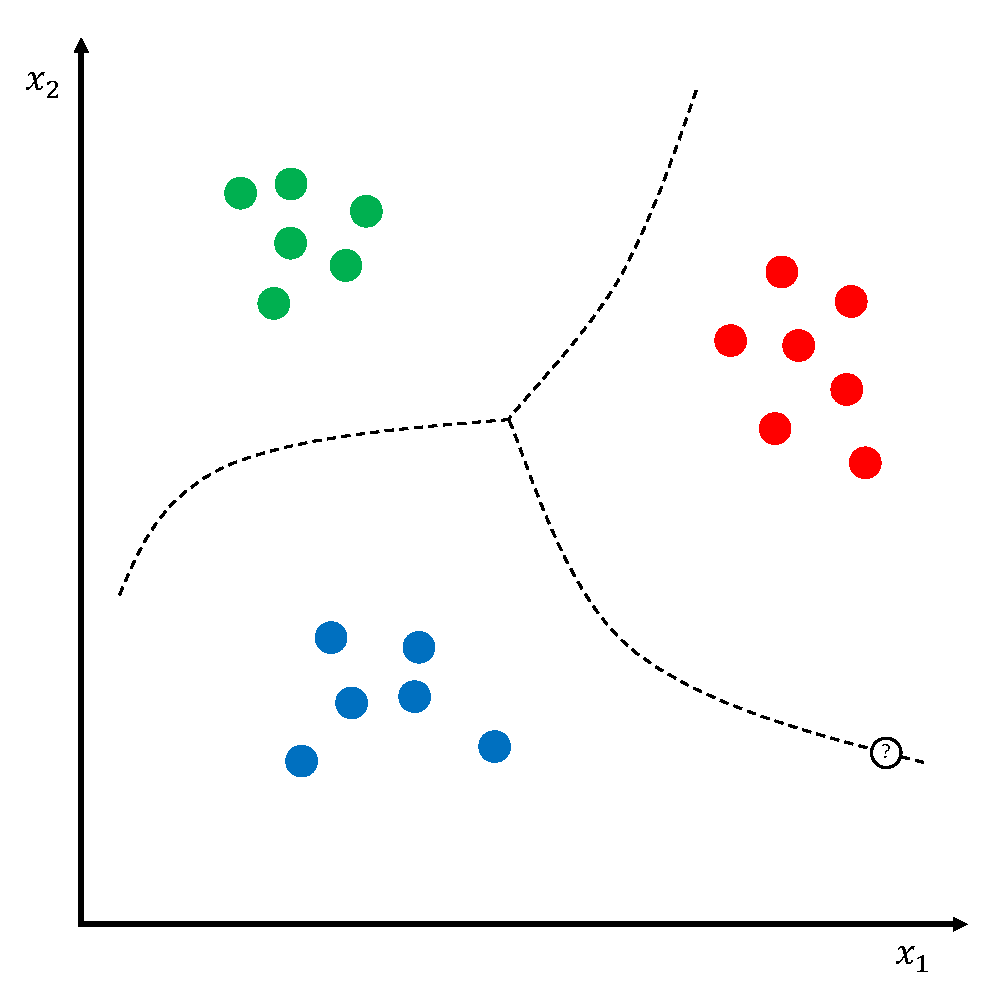
\includegraphics[width=210px]{figs/general/ml_example.pdf}
\caption{A toy example example of machine learning. This model learns to classify input data $\{x_1, x_2\}$ into three classes; red, green, and blue.}
\label{fig:mlex}
\end{figure}

The question of when transfer learning should be used can be answered by asking if {\slshape negative transfer} has occurred. {\slshape Negative transfer} is where the data from the source model leads to the reduced performance of the target model. In general, an example of when this can occur is when the two tasks are too dissimilar. In the context of hand tracking, it is important that the method used to achieve transfer learning is robust. In hand tracking, the occurance of {\slshape negative transfer} is determined by comparing how the model performs with real data versus synthetic data.

In terms of answering what to transfer, it is worth first reflecting on what the synthetic hand generation model is, and what the hand tracking model is. The synthetic hand generation model knows about the structure of the hand and how that is related to 3D space, and by giving it plausible articulations, that can be transferred to the hand tracking model.po Using the the terminology in \cite{pan2009survey}, the process of training a hand tracking system with synthetic data is an Inductive Transfer Learning task. In the context of this, the MANO model is the source task $\mathcal{T}_S$, and the target task $\mathcal{T}_T$ is the V2V-Posenet model. Both tasks have a common domain of human hands $\mathcal{D}$. A high level illustration of this concept is shown in Figure \ref{fig:ktex}.

%The source and target domains are both human hands, therefore they are the same, but the tasks are different. On a high level, the task of the MANO model is to generate a realistic synthetic representation of the human hand, the task of the V2V-Posenet model is to predict a set of keypoints from an inout mesh hand.

% MANO is learnt on a small amount of subjects and data, it uses the prior of the human, which is transferred to V2V.